
\label{sec:examples}

В ходе настоящей работы был создан комплекс программ для решения задачи выбора объектов, рассмотренной в разделе~\ref{selection_task}. Пользовательский интерфейс программного комплекса позволяет вводить экспертные оценки, задавать функцию качества объектов и т.\,д. Общая структура комплекса программ представлена на рис.~\ref{ris:program_global}, а скриншот пользовательского интерфейса представлен на рис.~\ref{ris:interface}.

Далее рассмотрим пример реального проекта, где применялся комплекс программ и где предложенная методика проведения экспертного опроса использовалась крупным российским инвестором для оценки инвестиционной привлекательности технологий, разрабатываемых в МГУ.

\begin{figure}[h]
\center{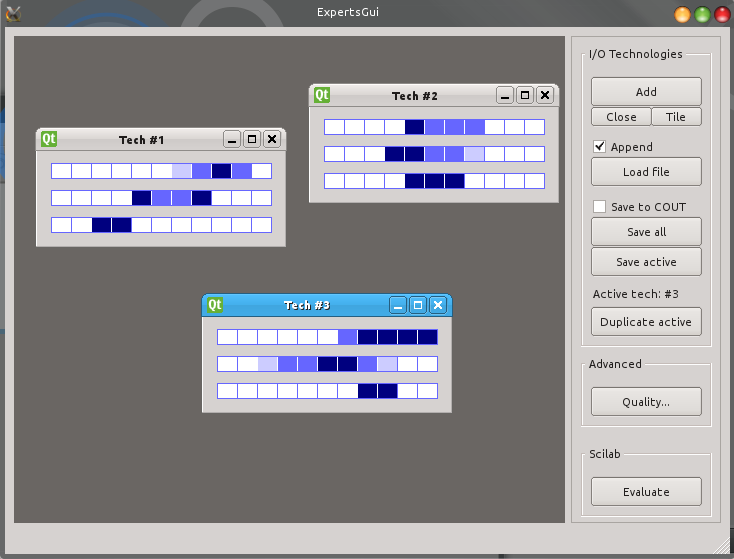
\includegraphics[width=0.85\linewidth]{./pic/combination6}}  
\caption{\small Скриншот пользовательсого интерфейса. Маленькие окошки соответствуют отдельным технологиям, а строчки квадратиков внутри них --- параметрам этих технологий. {\sl Здесь и далее на рисунках такого типа }: Сами квадратики символизируют баллы по шкале $X = \{0, 1, \ldots, 10\}$, а оттенок цвета конкретного квадратика --- возможность этого балла, по мнению эксперта (от белого, соответствующего возможности 0, до тёмно-синего, соответствующего возможности 1). }
\label{ris:interface}
\end{figure}

\subsection{Выбор наиболее привлекательных инновационных технологий}

%Этот пример построен вокруг реального проекта, где  %

Пусть имеется множество инновационных технологий $O$ размера $\abs{O} = N$.  Технология --- результат научно-технической деятельности, который включает в себя изобретения, промышленные образцы, компьютерные программы, технические данные или другие результаты интеллектуальной деятельности и может служить основой определённой практической, в том числе коммерческой деятельности. Каждая технология имеет одного или нескольких правообладателей, получающих выгоду от её применения в практической деятельности. Технологии являются инновационными в том смысле, что обладают значительной новизной и гипотетически имеют большой потенциал для развития, внедрения и получения прибыли, но всё это сопровождается значительным риском. 

%Если делать акцент не на самой технологии, а на команде людей, которые заняты разработкой и практическим применением технологии, то говорят об инновационном проекте или инновацонной компании. Всё, что ниже сказано про оценку технологий, остаётся верно и для оценки компаний с точностью до выбора критериев оценки.
%Есть крупный инвестор, у которого есть возможность стать совладельцем или полным владельцем технологии, если он вложит деньги и иные ресурсы в её развитие, вступив в сделку с текущими правообладателями. 
% (и так очевидно)

С точки зрения инвестора, технологии обладают разной инвестиционной привлекательностью, которая оценивается исходя из нескольких аспектов технологии, среди которых: доходность технологии через год после приобретения, её востребованность на рынке, конкурентоспособность, затраты на внедрение, потенциал интеллектуальной собственности, потенциал кадрового обеспечения, экологические риски, административные риски и т.\,д. 

Пусть привлекательность технологии по всем важным аспектам выражается числами $x_1 \in X_1, x_2 \in X_2, ...$, где мы для простоты положили $X_1 = X_2 = ... = \{0, ..., 10\}$. Инвестиционная привлекательность получается из этих чисел с помощью обычных операций сложения, перемножения и умножения на некоторые коэффициенты в соответствии со специально разработанной блок-схемой (рис.~\ref{ris:tech_scheme}), которая графически выражает функцию $f$, см. \eqref{e:function_f} на стр. \pageref{e:function_f}. 

\begin{figure}[h]
\center{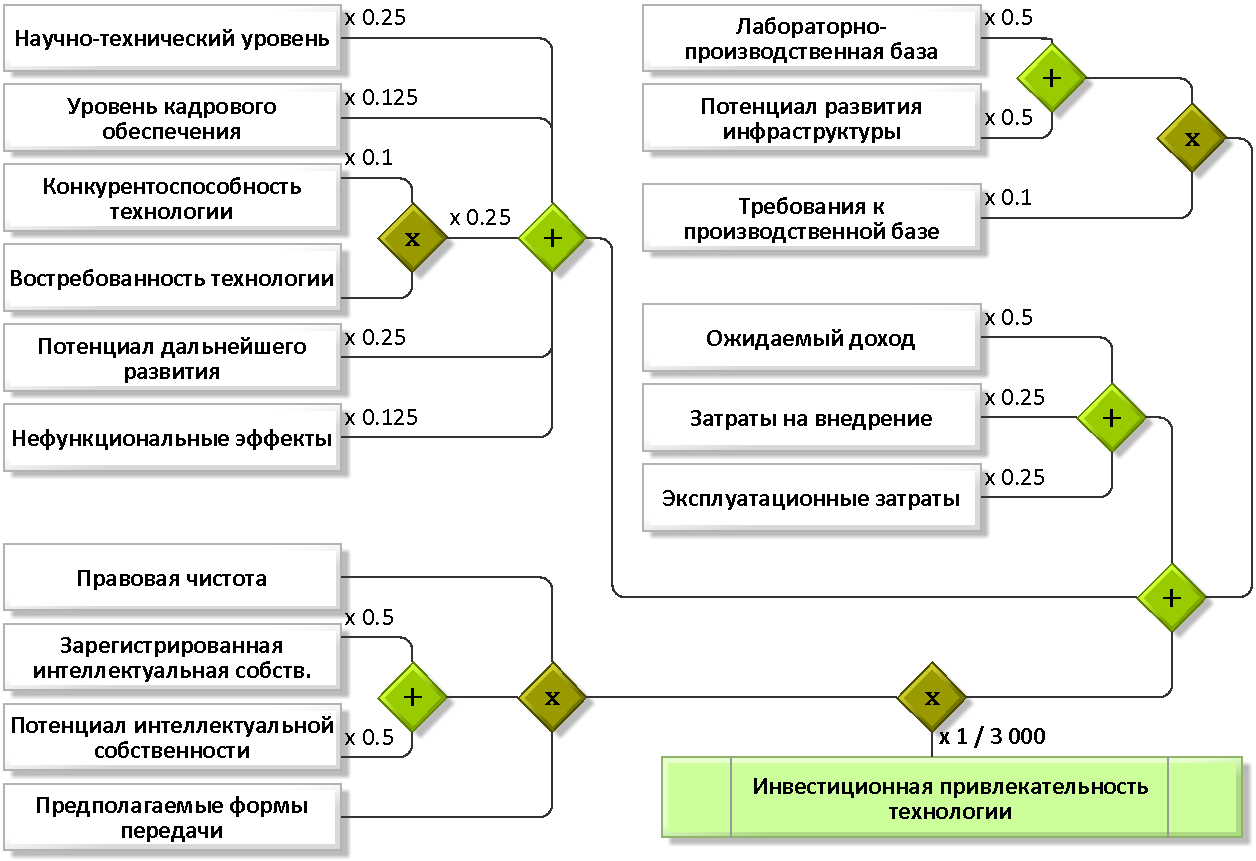
\includegraphics[width=0.85\linewidth]{./pic/schemeF2}}  
\caption{\small Блок-схема, иллюстрирующая конкретный вид функции $f$, объединяющей различные аспекты инновационной технологии, оцениваемые экспертом, в итоговую величину инвестиционной привлекательности технологии. }
\label{ris:tech_scheme}
\end{figure}

Были приглашены несколько экспертов. Каждого эксперта попросили оценить каждую технологию по каждому аспекту. Использовались нечёткие оценки, представленные в виде таблицы <<балл (значение $x \in \{0, ..., 10\}$) --- оценка (значение $p_{\tilde x}(x)$)>>, см.~рис.~\ref{ris:expert_sample}. В рассматриваемом случае выделялось $M = 16$ крупных аспектов с отдельными оценками. При этом с точки зрения методологии каждый из этих аспектов <<вобрал в себя>> ряд более мелких подпунктов примерно одинаковой важности, которые уже не требовали отдельных оценок во избежание чрезмерной нагрузки на эксперта. В документе-описании, который выдавался каждому эксперту, все аспекты расшифрованы: указано, какие подпункты мы рассматриваем и о чём следует  подумать перед выставлением оценки по каждому аспекту.
 
\begin{figure}[h]
\center{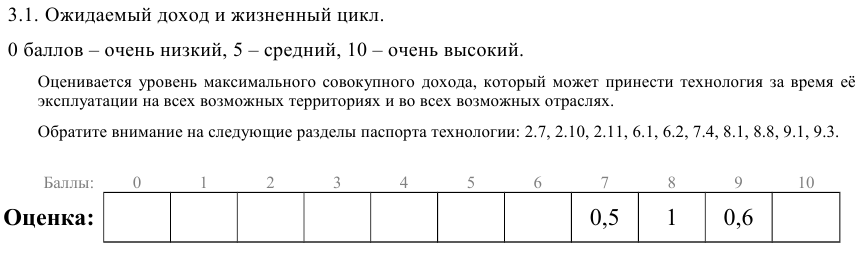
\includegraphics[width=0.85\linewidth]{./pic/expert_sample}}
\caption{\small Пример заполненного фрагмента листа экспертного опроса, проведённого по предложенной методике. Эксперт выставил нечёткую оценку в ячейках таблицы <<балл (значение $x$) --- оценка (значение $p(x)$)>>. Пустым клеткам таблицы соответствуют значения $p(x) = 0$. }
\label{ris:expert_sample}
\end{figure}

Интересно отметить, что для различных рисков и других негативных аспектов технологии большие числовые значения в таблице интуитивно соответствуют более плохой ситуации, более низкому качеству объекта. Но поскольку $f$ должна быть монотонна по всем аргументам, требуется единообразие, например, увеличение аргументов $f$  всегда приводит к более высокому значению $f$, т.\,е. более высокому качеству. Поэтому были сделаны дополнительные указания для экспертов в тех местах, где большие числовые значения интерпретируются как более низкий риск. Этого можно избежать, если делать предварительную обработку оценок: автоматически отразить оценки, нарушающие монотонность, вдоль оси абсцисс (баллов) вокруг оси, проходящей через середину диапазона баллов.

Совокупность сырых экспертных оценок была загружена в программу расчёта коллективной оценки. Полученное коллективное мнение было загружено в программу, реализующую быстрый алгоритм нахождения возможности не попасть в $k$ лидеров для каждой из технологий, которых в рассматриваемом случае набралось $N = 15$ штук. Программа расчёта оптимального решения была запущена при разных значениях $k = 1, 2, \ldots, N$, в результате чего обнаружилось, что только при $k=2, 14$ можно сделать однозначный выбор технологий, опираясь на полученное оптимальное решение.  

\begin{figure}[h]
\center{ \resizebox{0.5\linewidth}{!}{\showevDisplayFullScale{./pic/realScaled13.txt}} }
\caption{\small Технология-аутсайдер на реальных экспертных данных в проекте по заказу крупного российского инвестора. Строчки квадратиков символизируют параметры технологии. Легенду цветовых оттенков см. под рис.~\ref{ris:interface}.}
\label{ris:tech_13}
\end{figure}

В случае $k = 14$ оптимальный выбор состоит из всех технологии, кроме одной, показанной на риc.~\ref{ris:tech_13}. Эта технология-аутсайдер на вид не так уж плоха, но обратите внимание на последние несколько параметров --- по ним выставлены довольно низкие оценки, а в используемую функциею качества последние $4$ параметра входят мультипликативно (рис.~\ref{ris:tech_scheme}) и сильно влияют на итоговое качество технологии.

Результат работы программы оправдал ожидания в следующем смысле. В рассматриваемом проекте выполнялся предварительных отбор наименее качественных технологий, и на детальную экспертизу выносились технологии, приблизительно равные по ожидаемому экспертами качеству. Отсюда понятно, что большинство технологий-лидеров не разделяются однозначно. Получилось, что при желании выбрать небольшое число технологий-победителей для трансфера (покупки), разумно остановиться на $k=2$ технологиях. 

\subsection{Примеры, демонстрирующие преимущество нечётких оценок в задаче выбора объектов}

Рассмотрим примеры, демонстрирующие преимущество нечётких экспертных оценок перед оценками других типов в задаче выбора объектов, а также сравним подходы к вычислению коллективной экспертизы.
\begin{example}
\label{two_dressings_basic}
Предположим, имеются $2$ эксперта, каждый из которых оценивает $3$ объекта. Пусть, для простоты примера, каждый объект моделируется только одним нечётким элементом $\tilde x_i,\ i=1,2,3$, полностью характеризующим его качество, а выставляемые экспертами значения возможности событий вида  $\{\tilde x_i = x\},\ x \in X$ ограничиваются двухточечным множеством $\{0, 1\}$. Допустим теперь, что эксперты выставили оценки, как показано на рис.~\ref{two_dressings_source}.
\end{example}

\begin{figure}[h]
\center{
\resizebox{0.45\linewidth}{!}{\showevDisplay{./pic/sample1/ex1.txt}}
\resizebox{0.45\linewidth}{!}{\showevDisplay{./pic/sample1/ex2.txt}}
}
\caption{\small Экспертные оценки $3$-х объектов от первого эксперта (слева) и второго эксперта (справа) к примеру~\ref{two_dressings_basic}. Легенду цветовых оттенков см. под рис.~\ref{ris:interface}. }
\label{two_dressings_source}
\end{figure}

Упорядоченность объектов по качеству в случае использования лишь <<$\delta$-образных>> оценок устанавливается очень просто: достаточно сравнить значения качества, которым приписана единичная возможность, для разных объектов. Следуя этой логике, заметим, что упорядоченность, основанная на оценках первого эксперта, есть $1, 2, 3$, а упорядоченность, основанная на оценках второго эксперта --- $3, 2, 1$. Теперь рассмотрим среднее арфиметическое экспертных оценок и их супремум, изображенные на рис.~\ref{two_dressings_mean}.

\begin{figure}[h]
\center{
\resizebox{0.45\linewidth}{!}{\showevDisplay{./pic/sample1/mean.txt}}
\resizebox{0.45\linewidth}{!}{\showevDisplay{./pic/sample1/sup.txt}}
}
\caption{\small Среднее арифметическое (слева) и супремум (справа) экспертных оценок с рис.~\ref{two_dressings_source} к примеру~\ref{two_dressings_basic}. Поскольку значения возможностей в рассматриваемом примере лежат на множестве $\{0, 1\}$, то супремум есть просто объединение носителей распределений. А среднее арифметическое получено усреднением значений качества, которым приписана единичная возможность.}
\label{two_dressings_mean}
\end{figure}

Среднее арифметическое на рис.~\ref{two_dressings_mean}, слева, на самом деле, моделирует использование не нечёткх, а балльных оценок, или оценок первого типа из раздела~\ref{sec:math_methods_global}. А именно, если бы эксперты $r=1,2$ выставили просто те баллы $x_i^{(r)}$ для объектов $i=1,2,3$, которые отмечены тёмно-синим цветом на рис.~\ref{two_dressings_mean}, слева, то стандартная процедура нахождения коллективного мнения балльных оценок на практике состояла бы в вычислении средних баллов $\bar{x}_i$. 

Но упорядоченность объектов по качеству, полученная с использованием среднего арифметического экспертных оценок, есть $2, 3, 1$, что противоречит мнению как первого, так и второго экспертов. Это означает, что использовать среднее арифметическое в качестве коллективного мнения экспертов в рассматриваемом случае {\sl неприемлимо}.

С другой стороны, если вернуться к нечётким экспертным оценкам и использовать супремум в качестве коллективного мнения экспертов, картина получается другая. Оказывается, решение задачи выбора одного или двух из трёх объектов в случае использования супремума с рис.~\ref{two_dressings_mean}, справа, не единственно, причём возможность ошибиться, выбрав $i$-й объект, равна единице для всех $i$. Последнее служит индикатором того, что противоречие между мнениями экспертов <<слишком сильное>>.

На тот же набор экспертных оценок можно посмотреть и под другим углом.
\begin{example}
\label{two_dressings_basic2}
Предположим теперь, имеется только один эксперт. Однако, ситуация такова, что для рассматриваемых объектов возможны два сценария развития, в соответствии с которыми качество объектов может быть оценено либо как на рис.~\ref{two_dressings_source} слева, либо как на том же рисунке справа. Что делать эксперту?
\end{example}

Если эксперт ограничен использованием балльных оценок, взаимно однозначно сопоставленных <<$\delta$-образным>> нечётким оценкам, то он может или ответить как на рис.~\ref{two_dressings_source} слева или справа, или выбрать некий <<промежуточный>> вариант, например как на рис.~\ref{two_dressings_mean} слева. Во всех случаях будет получаться различная упорядоченность объектов по качеству (см. пример~\ref{two_dressings_basic}). Если же дать эксперту возможность использовать всю мощь нечётких оценок, он может просто выбрать и тот, и другой сценарий развития объектов, ответив так, как на  рис.~\ref{two_dressings_mean} справа. Эта неопределённость, присущая объектам {\sl по мнению эксперта}, сразу же отразится на решении задачи выбора как неединственность решения.

Рассмотрим, наконец, сравнение методов вычисления коллективного мнения экспертов с помощью векторов предпочтений и с помощью вычисления верхней грани возможностных распределений (см. раздел~\ref{collective_global}).
\begin{example}
\label{vector_sup_comparison_sample}
Пусть имеется $3$ эксперта, и каждый выдаёт одно экспертное мнение $p_r(\cdot),\ r=1,2,3$. Они изображены на рис.~\ref{vector_sup_comparison_pic}, причём $\p_1(\cdot) = \p_2(\cdot) \neq \p_3(\cdot)$. На том же рисунке представлены: средняя оценка $\bar{\p}(\cdot)$, полученная по методу векторов предпочтений и супремум $\check{\p}(\cdot) = \vee p_r(\cdot)$, $r=1,2,3$. Заметен кумулятивный характер экспертной оценки $\bar{\p}(\cdot)$: она имеет более высокий максимум в той части области определения, где сходятся во мнениях два из трёх экспертов. Однако, максимумы $\bar{\p}(\cdot)$ и максимумы $p_r(\cdot),\ r=1,2,3$ не совпадают. Что касается супремума $\check{\p}(\cdot)$, то он <<стремится выравнять>> по значениям возможности все возможные элементарные события в том случае, когда экспертные оценки <<сильно несогласованы>>, как в рассматриваемом примере. Такое поведение супремума следует из его определения и алгоритма его вычисления в разделе~\ref{easy_collective_sup}.  
\end{example}

\begin{figure}[h]
\center{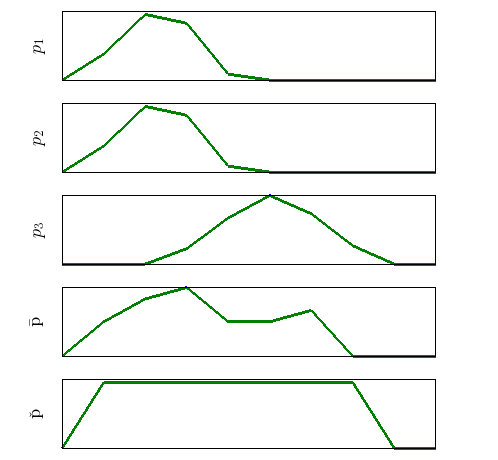
\includegraphics[width=0.85\linewidth]{./pic/prefsup102}}
\caption{\small Иллюстрация экспертных мнений $p_r(\cdot),\ r=1,2,3$, их среднего по методу векторов предпочтений $\bar{\p}(\cdot)$ и супремум $\check{\p}(\cdot)$ к примеру~\ref{vector_sup_comparison_sample}.}
\label{vector_sup_comparison_pic}
\end{figure}

%\todo[inline]{Ещё есть косяки в списке литературы. Например, в [1]~--- <<Владимировна Ф. О.>>, в [2]~--- <<Пытьев Ю.>> без <<П.>>. }


\begin{comment}	      
	      \\ \hspace{2ex} Ранжировка (Э1): $1, 2, 3$.
		  \\ \vspace{1ex}
	    
	      \\ \hspace{2ex} Ранжировка (Э2): $3, 2, 1$.	      
		  \\ \vspace{1ex}
	      \resizebox{0.9\linewidth}{!}{\showevDisplayRough{./pic/sample1/mean.txt}}
	      \\ \hspace{2ex}  Ранжировка (среднее): $2, 3, 1$.
		  \\ \vspace{1ex}
	      \resizebox{0.9\linewidth}{!}{\showevDisplayRough{./pic/sample1/sup.txt}}
	      \\ \hspace{2ex} Ранжировка (супремум): \textbf{?}	
	      


\subsection{Пример 2: Выбор оптимальных реактивов для маркировки белков в цикле ***}

Этот пример посвящён важной области применения экспертных опросов на стыке естественных наук и экономики --- области планирования эксперимента. 

Одним из центральных вопросов для науки биохимии является вопрос о том, какие химические реакции протекают в живом организме, и какие вещества участвуют в этих реакциях. Как правило, исследуют т.\,н. циклы реакций с участием белков. В живом организме встречается много тысяч различных белков и добрая сотня из них участвует в исследуемом цикле реакций. Концентрация веществ, участвующих в реакциях, в частности -- белков, как правило, изменяется на отдельных стадиях цикла реакций, и может изменяться в результате полного цикла.

Для идентификации конкретного белка и определения его концентрации служат специальные реактивы, причём один реактив может обладать активностью сразу к нескольким белкам (и заранее неизвестно, к каким?). Биологи контролируют изменение концентрации выбранных белков в некоторой точке организма таким образом, что организм не погибает (и вмешательство в его работу минимально?) По каждому белку есть предположения относительно того, насколько возможно, что: (1) его количество уменьшится, (2) не изменится, (3) увеличится. В силу некоторых причин, в том числе, но не ограничиваясь дороговизной реактивов, мы можем контролировать только небольшое количество белков, как правило, в пределах $10$.

Объекты -- белки. <<Качество>> белка складывается из того, какие белки, по мнению эксперта, участвуют в цикле (и их имеет смысл контролировать), и насколько дорогой реактив требуется для контроля. Эксперт оценивает для каждого белка $i \in \setN$ возможность $\p_{ij}(x)$ обнаружения изменения его концентрации на $x$ процентов (или чего там, логарифма какого-нибудь) с помощью реактива $j \in \setM$. Цены различных реактивов учтены в $f(\cdot)$ как коэффициенты перед $x_{ij}$ для разных $j$.

%Объекты -- реактивы. <<Качество>> реактивов складывается из того, какие белки, по мнению эксперта, участвуют в цикле. Эксперт оценивает для каждого реактива $i \in \setN$ возможность $\p_{ij} обнаружения каждого белка $j \in \setM$ (довольно много оценок, трудно для эксперта?). Нечёткий вектор $\theta: \p_{\theta} = \inf \p_{ij}$ не имеет смысла, т.\,к. (а) я забыл про баллы, ещё одно измерение и (б) при таком выборе нет независимости компонент, потому что есть априорные возможности обнаружить белок в реакции идеальным реактивом.    

%Выбор измерительного прибора мы будем рассматривать в контексте теории измерительно-вычислительнх преобразователей как средств измерений (ИВП) Ю.~П.~Пытьева \cite{4}. 
\end{comment}


